\documentclass[a4paper]{article}

\usepackage[utf8]{inputenc}
\usepackage{geometry}

\usepackage{float}
\usepackage{graphicx}
\usepackage{lipsum} 
\usepackage{xcolor} 
\usepackage[hidelinks]{hyperref}
\usepackage{multirow}

\usepackage{caption}
\usepackage{float}
\usepackage{mathtools}

\usepackage{titlesec}

\usepackage{natbib}

\geometry{
  top=1.2in,
  bottom=1.5in,
  left=1.1in,
  right=1.1in,
  headheight=10pt,
  headsep=10pt,
  footskip=50pt
}


\titleformat{\section}       % Command to format sections
  {\normalfont\bfseries\fontsize{9}{10}\selectfont}          % Font size and style for section titles
  {\thesection}              % Section number format
  {0.5em}                      % Spacing between number and title
  {}                         % Code before the title

\titleformat{\subsection}  % Command to format subsections
  {\normalfont\bfseries\fontsize{9}{10}\selectfont}  % Font size and style for subsection titles
  {\thesubsection}          % Subsection number format
  {0.5em}                   % Spacing between number and title
  {}                        % Code before the title


  
% Tags for the mat expressions, use [] instead
\newtagform{brackets}{[}{]}
\usetagform{brackets}

\captionsetup[figure]{labelfont=bf}  % This will make "Figure 1:" bold

\renewcommand{\refname}{}

\begin{document}

\noindent
\textbf{Psychological Factors and COVID-19 Test Outcomes: Associations and Differences}\\
\vspace{0.1em} 
\noindent\hrulefill 
\vspace{0.8em} 

\begin{center}
    \textbf{Eurico Martins, Gutelvam Fernandes, Hugo Alves}\\
    \vspace{0.5em}
    Master in Applied Artificial Intelligence;\\
		EST - Instituto Politécnico do Cávado e do Ave, Portugal.\\
    \vspace{0.5em}
    \href{mailto:a8794@alunos.ipca.pt}{a8794@alunos.ipca.pt}, \href{mailto:a33791@alunos.ipca.pt}{a33791@alunos.ipca.pt}, \href{mailto:a30783@alunos.ipca.pt}{a30783@alunos.ipca.pt}
\end{center}

\vspace{3em}
\noindent {\bfseries \fontsize{9}{11}\selectfont ABSTRACT}
\vspace{1em}\newline
This study investigates the relationship between psychological factors—stress, anxiety, depression, and optimism—and COVID-19 test outcomes.
Correlation analyses identified significant associations among the psychological variables, though their correlations with testing positive for COVID-19 were weak.
Stress, anxiety and depression exhibited minimal negative associations, while optimism demonstrated a positive correlation with positive test results.
Normality tests revealed deviations from normality, and Mann-Whitney U tests indicated significant group differences in stress, depression, and optimism,
while anxiety showed no statistically significant difference. These findings highlight nuanced links between psychological health and COVID-19 testing outcomes.

\vspace{1em}
\textbf{Keywords}: Psychological factors, stress, anxiety, depression, optimism, COVID-19.

\vspace{2em}
\section{INTRODUCTION}
\vspace{0.5em}
The COVID-19 pandemic has had a profound impact on both physical and mental health worldwide.\newline
While the physical health consequences are well-documented, the psychological effects have also been significant, with heightened levels of depression, anxiety, and stress reported across the globe.
Social isolation, economic uncertainty, and ongoing health fears have all contributed to a marked increase in mental health challenges, exacerbating existing vulnerabilities (\citet{PsychologicalImpactQuarantine}).
The pandemic disrupted daily routines, created widespread financial and social stress, and fostered an environment of uncertainty, leading to substantial deterioration in psychological well-being for many individuals.
\vspace{0.5em}\newline
Depression emerged as one of the most prevalent psychological effects of the pandemic (\citet{PrevalenceDepressionDuringCOVID-19}).
Social isolation, coupled with uncertainty surrounding the virus, intensified feelings of helplessness and loneliness.
Economic challenges, such as job losses and financial insecurity, further contributed to the surge in depressive symptoms.
The necessary social distancing measures, though essential for preventing virus spread,
left many without the support systems that might have helped mitigate feelings of isolation, leading to a global rise in depression during the pandemic.
\vspace{0.5em}\newline
Anxiety also became a major issue, driven by the constant flow of information about the virus and the fear of its unpredictable impact on health (\citet{Frontiers2021StressAnxietyEconomicInsecurity}).
The concern about personal and familial well-being, along with economic instability, led to heightened anxiety levels.
Unlike transient anxiety, the persistent nature of the pandemic resulted in chronic distress, affecting individuals' ability to cope with daily life and function normally.
These prolonged periods of anxiety added to the overall mental health burden of the crisis.
\vspace{0.5em}\newline
Dispositional optimism, or the general expectation that good things will happen, emerged as a key protective factor against the mental health challenges of the pandemic (\citet{Carver2010WileyInterdisciplinaryReviews}).
Optimistic individuals tend to cope with adversity in more adaptive ways, maintaining a sense of hope and agency during difficult times.
Research has shown that optimism is associated with better psychological outcomes, including lower stress levels and greater resilience (\citet{Lee2019OptimismLongevity}). During the pandemic,
optimism allowed individuals to manage uncertainty more effectively, promoting healthier behaviors and improving overall well-being.
\vspace{0.5em}\newline
Stress, an inevitable response to perceived challenges, has been another significant consequence of the pandemic.
The disruption of daily life, fear of illness, and uncertainty about the future combined to create a chronic state of stress for many (\citet{Cohen2016PsychologicalStressDisease}).
Prolonged stress has been linked to various physical and mental health issues,
including cardiovascular problems and weakened immune systems, further exacerbating the psychological toll of the pandemic.
The persistent nature of stress during this period has contributed to a rise in stress-related disorders globally (\citet{NIMH2023StressImpactCOVID}).
\vspace{0.5em}\newline
The intersection of COVID-19 with mental health issues like depression, anxiety, and stress highlights the need for psychological resilience.
While the pandemic has undeniably worsened global mental health, optimism has proven to be a key factor in mitigating its effects (\citet{Conversano2020MindfulnessResilience}). Further research into 
how optimism influences mental health could offer valuable strategies to strengthen resilience and better equip individuals to cope with the ongoing challenges posed by global crises.


\vspace{2em}
\section{METHODS}
\subsection{Theoretical Framework}
\vspace{0.5em}
This was a descriptive observational study utilizing an existing dataset of 193 COVID-19 individuals.
The dataset included a range of demographic, behavioral, and psychological variables.
The primary objective of the study was to investigate the relationship between psychological factors — depression, anxiety, stress, and optimism — and COVID-19 test outcomes.

\vspace{1em}
\subsection{Research Methodology}
\vspace{0.5em}
This study will employ a descriptive observational design to analyze the relationship between COVID-19 test status (positive vs. negative) and psychological factors,
including stress, anxiety, depression, and optimism.
\vspace{0.5em}\newline
The methodology will focus on a comprehensive descriptive analysis, normality testing, and appropriate non-parametric statistical methods to address the research aims.
The analysis will begin with a descriptive statistical examination of each variable. Measures such as means, medians, standard deviations, and interquartile ranges will be calculated to summarize the psychological factors and COVID-19 test outcomes.
To determine the distribution of the data, normality tests such as the Kolmogorov-Smirnov test will be applied.
\vspace{0.5em}\newline
Given the expected non-normal distribution of the data, Spearman’s rank correlation coefficient will be used to assess the relationships between psychological variables (stress, anxiety, depression, and optimism) and their association with COVID-19 test status.
Spearman’s method is well-suited for identifying monotonic relationships in non-normally distributed data.
\vspace{0.5em}\newline
To further analyze differences between COVID-19 test groups (positive vs. negative), the Mann-Whitney U test will be performed. This non-parametric test will evaluate whether there are significant differences in psychological factors between the two groups. Statistical significance will be set at 
\(\boldsymbol{p < 0.05 }\), and all analyses will be conducted using appropriate statistical software, such as SPSS.
\vspace{0.5em}\newline
By combining descriptive analysis, normality testing, correlation analysis, and group comparisons, this methodology ensures a robust examination of the relationship between COVID-19 status and psychological factors, addressing the research question effectively within the constraints of the data.


\vspace{1em}
\subsection{Statistical Analysis}
\vspace{0.5em}
The analysis of the dataset in relation to the psychological factors—stress, anxiety, depression, and optimism—reveals interesting insights into their potential influence on COVID-19 test status.
The Spearman correlation results suggest significant associations between various psychological variables, but the relationship with COVID-19 status is relatively weak,
especially when considering the null hypothesis that psychological factors are unrelated to having tested positive or negative for COVID-19.
\vspace{0.5em}\newline
The descriptive statistics reveal key insights into the sample \textit{(Figure \ref{fig:descriptiveSts})}. 
The mean stress level is 5.40, with moderate variability and a slightly right-skewed distribution. Anxiety, with a mean of 2.85, exhibits a highly right-skewed distribution and a pronounced peak,
indicating that while most participants reported low anxiety, a few experienced very high levels.
Depression, with a mean of 4.77, also shows a right-skewed distribution, though less pronounced than anxiety.
In contrast, optimism has a mean of 19.52 and a nearly normal distribution, suggesting relatively consistent levels of optimism among participants.\newline
The mean age is 29.15 years, with a slight right skew, reflecting a younger sample.
Only 28\% of participants tested positive for COVID-19, with a skewed distribution toward negative cases.\newline
In summary, while stress, anxiety, and depression show moderate variability with skewed distributions, optimism appears more consistent and normally distributed.\newline 
The relatively high mean for stress (5.40) and the skewed distributions for anxiety and depression suggest that while most participants report moderate
to low levels of these psychological factors, there are some who experience notably higher levels.
The consistency in optimism scores, with a nearly normal distribution, contrasts with the variability observed in stress, anxiety, and depression.\newline
The sample's younger age and the predominance of participants who tested negative for COVID-19 may influence the interpretation of these psychological factors,
as these variables could interact with COVID-19 status and psychological well-being.\newline
These trends offer valuable context for understanding the psychological profiles within the sample.
\vspace{1.5em}

\begin{figure}[ht]
  \centering
  \caption{Descriptive Statistics and Normality Tests}
  \label{fig:descriptiveSts}
  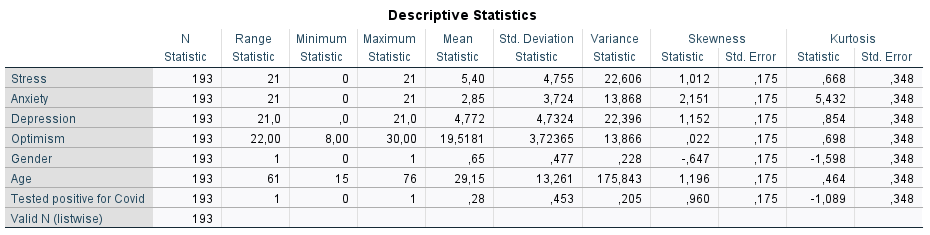
\includegraphics[width=\textwidth]{img/descriptive_statistics.png}  % Adjust the file name and extension as necessary
\end{figure}

\vspace{3em}
\noindent
The normality test results assess whether the distributions of stress, anxiety, depression, and optimism are normally distributed,
separately for participants who tested positive and those who tested negative for COVID-19.
The Kolmogorov-Smirnov test is used to assess whether a sample distribution differs significantly from a reference distribution,
particularly for larger sample sizes (typically more than 50) to ensure reliable results. \textit{(Figure \ref{fig:normalityTest})}.
\vspace{0.5em}\newline
The Kolmogorov-Smirnov test results reveal significant deviations from normality for all variables in the sample,
with p-values less than \(\boldsymbol{0.001}\) for stress, anxiety, depression, optimism, and COVID-19 test status.
These findings confirm that none of the variables follow a normal distribution, supporting the use of non-parametric statistical methods,
such as Spearman correlations and Mann-Whitney U tests, for further analysis.
\vspace{1.5em}

\begin{figure}[H]
  \centering
  \caption{Normality Tests}
  \label{fig:normalityTest}
  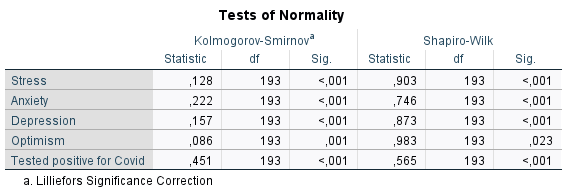
\includegraphics[width=\textwidth]{img/normality_test.png}  % Adjust the file name and extension as necessary
\end{figure}


\vspace{3em}
\noindent
With the psychological variables, stress is significantly correlated with both anxiety and depression (\(\boldsymbol{r = 0.774, p < 0.001}\) and \(\boldsymbol{r = 0.807, p < 0.001}\), respectively),
as assessed using the Spearman's rho correlation test \textit{(Figure \ref{fig:correlationsTest})}.\newline
This indicates that individuals experiencing higher levels of stress are more likely to report higher levels of anxiety and depression.
Additionally, optimism shows negative correlations with stress, anxiety, and depression (\(\boldsymbol{r = -0.375, r = -0.392}\), and \(\boldsymbol{r = -0.496}\), respectively),
suggesting that individuals with lower levels of optimism tend to experience higher levels of stress, anxiety, and depression.
\vspace{0.5em}\newline
These correlations, however, are not entirely surprising given the established links between these psychological factors in the broader literature.
\vspace{0.5em}\newline
When considering the influence of these psychological factors on COVID-19 test results, the correlations with the variable Tested positive for Covid are relatively weak.\newline
Stress shows a small negative correlation (\(\boldsymbol{r = -0.148, p = 0.041}\)), which suggests a very modest inverse relationship between stress levels and testing positive for COVID-19.
However, this correlation is far from strong and does not provide evidence to support a significant psychological influence on COVID-19 status.\newline
Similarly, anxiety (\(\boldsymbol{r = -0.108, p = 0.134}\)) and depression (\(\boldsymbol{r = -0.201, p = 0.005}\)) also show weak negative correlations with COVID-19 test results,
indicating that higher levels of anxiety and depression may be slightly more common in individuals who test negative, though these relationships are still modest in size.
\vspace{0.5em}\newline
On the other hand, optimism is positively correlated with testing positive for COVID-19 (\(\boldsymbol{r = 0.237}\), \(\boldsymbol{p < 0.001}\)), suggesting a small but significant relationship between higher optimism and a higher likelihood of testing positive for the virus.\newline
This finding suggests an intriguing, though modest, pattern, but it’s important to note that it doesn’t establish a cause-and-effect relationship.
\vspace{0.5em}\newline
Therefore, while significant correlations between psychological variables themselves exist, the relationship between these variables and the likelihood of testing positive for COVID-19 remains weak.
The correlation between optimism and testing positive for COVID-19 is the only significant finding, although it is small in magnitude.
\vspace{0.5em}\newline
This analysis suggests that while psychological factors are undeniably interconnected, their influence on COVID-19 test outcomes is \textbf{minimal}, supporting the \textbf{null hypothesis} that stress, anxiety,
depression, and optimism do \textbf{not significantly affect} the likelihood of testing positive for the virus.
\vspace{1.5em}


\begin{figure}[ht]
  \centering
  \caption{Corelatuib Spearman's rho Test}
  \label{fig:correlationsTest}
  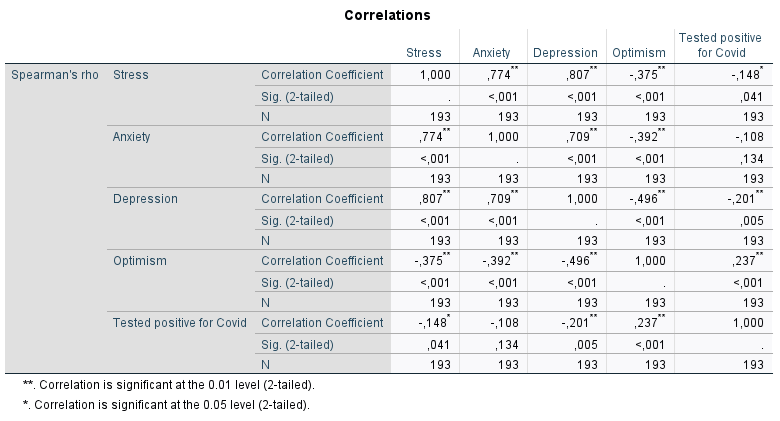
\includegraphics[width=\textwidth]{img/correlations.png}  % Adjust the file name and extension as necessary
\end{figure}

\vspace{3em}\noindent
The Mann-Whitney U test \textit{(Figure \ref{fig:mannWhitney})} evaluates differences between participants who tested positive for COVID-19 and those who tested negative.
This non-parametric test is appropriate as the data do not meet the assumptions of normality.\newline
For stress, the p-value is 0.041, indicating a statistically significant difference between groups at the \(\boldsymbol{\alpha = 0.05}\) level,
suggesting that participants who tested negative for COVID-19 report slightly higher stress levels.
Anxiety, however, shows no significant difference, with a p-value of \(\boldsymbol{0.133}\), indicating no meaningful variation between the two groups.
Depression has a p-value of \(\boldsymbol{0.005}\), revealing a statistically significant difference, suggesting that participants who tested negative for COVID-19 experience higher levels of depression.
Optimism, with a p-value of 0.001, also shows a significant difference, with participants who tested positive for COVID-19 reporting higher levels of optimism.
\vspace{0.5em}\newline
In summary, while stress, depression, and optimism show significant differences between groups, the effect sizes appear modest.
Anxiety does not differ significantly between those who tested positive and negative for COVID-19.

\begin{figure}[H]
  \centering
  \caption{Mann-Whitney U Test}
  \label{fig:mannWhitney}
  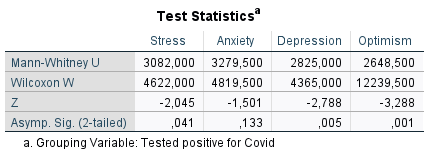
\includegraphics[width=0.75\textwidth]{img/mann-whitney.png}  % Adjust the file name and extension as necessary
\end{figure}

\setlength{\textfloatsep}{50pt}
\section{CONCLUSION}
\vspace{0.5em}

\noindent
This study aimed to explore the relationship between psychological factors like stress, anxiety, depression, and optimism and COVID-19 test outcomes in a sample of 193 individuals.\newline
The results offer insights into the interconnectedness of these psychological variables and their potential influence on COVID-19 status, though the overall findings point to minimal effects.
\vspace{0.5em}\newline
While stress, anxiety, and depression showed significant correlations with each other, indicating a strong interrelationship, the correlations with COVID-19 test outcomes were weak.
Notably, optimism was the only psychological variable that showed a significant positive correlation with testing positive for COVID-19.
\vspace{0.5em}\newline
However, the relationship between optimism and COVID-19 test status was small, suggesting that individuals with higher optimism were slightly more likely to test positive.
This finding, though statistically significant, does not imply a causal relationship, as the effect size remains modest.
\vspace{0.5em}\newline
The normality tests confirmed that most psychological variables, including stress, anxiety, and depression, deviated significantly from normal distribution,
justifying the use of non-parametric statistical methods such as Spearman’s rho correlation and the Mann-Whitney U test.
The Mann-Whitney U test results indicated that participants who tested negative for COVID-19 reported slightly higher levels of stress and depression,
while those who tested positive for the virus reported higher levels of optimism.
\vspace{0.5em}\newline
In summary, while there are significant correlations between psychological variables, their impact on COVID-19 test outcomes is limited. The study supports the null hypothesis, indicating that psychological factors such as stress, anxiety, depression, and optimism do not significantly affect the likelihood of testing positive for COVID-19.

\newpage
\section{REFERENCES}

\bibliographystyle{apalike}
\bibliography{refs}

\end{document}